\section{Introduction}

\begin{frame}[fragile, allowframebreaks]{Introduction}

\begin{block}{Acknowledgement}
A special thanks to {\bf CeSeNA Security} group and \emph{Marco Ramilli} our ``old'' mentor...
\end{block}

\begin{block}{Where to find us}
\begin{itemize}
\item Website: {\small \url{http://cesena.ing2.unibo.it/}}
\item Facebook: {\small \url{https://www.facebook.com/groups/105136176187559/} }
\item G+: {\small \url{https://plus.google.com/communities/101402441314003721224}}
\end{itemize}
\end{block}

\framebreak

\begin{block}{Before smashing things}
We need to say some words about security in general :) !
\end{block}

\framebreak

\begin{block}{Security facts in modern era}
\begin{itemize}
\item Each security breach costs over 500k to Corporates\\ 
{\small \url{http://goo.gl/RAUgOg}}
\item Cyber-Security market is growing (\emph{63 billion in 2011, 120 billions in 2017})\\ {\small \url{http://goo.gl/Zq8Efj}}
\item Zero-Day exploit black markets, and Bug-Bounty (\emph{yes Microsoft is doing it too})
\end{itemize}
\end{block}

\framebreak

\begin{block}{Is someone still using C}
Lot of C/C++ out there.. {\small \url{http://langpop.com/}  \url{http://www.tiobe.com/} }
\end{block}

\begin{block}{Buffer OverFlows are old stuff}
\begin{center}
\begin{tabular}{l|c}
\hline
Who  & \emph{NGINX Web server} \\
\hline 
What & \emph{stack-based buffer overflow} \\
\hline
When & \emph{ \Large \bf \color{red} 2013 } \\
\hline
\end{tabular}
\end{center}
\hfill Really??\\
\hfill \emph{Check this CVE: \url{http://goo.gl/4cIBqI}}
\end{block}

\end{frame}

\subsection{Smashing the stack}

\begin{frame}[fragile, allowframebreaks]{Smash the stack}
\begin{block}{\emph{Smash The Stack} [C programming] n.}
\begin{itemize}
\item On many C implementations it is possible to {\bf corrupt the execution stack} by \underline{writing past the end of an array} declared auto in a routine.
\item Code that does this is said to smash the stack, and \emph{can cause return from the routine to jump to a random address}.
\end{itemize}
\begin{center}
\bf This can produce some of the most insidious data-dependent bugs known to mankind.
\end{center}
\end{block}
\end{frame}
%%%%%%%%%%%%%%%%%%%%%%%%%%%%%%%%%%%%%%%%%%%%%%%%%%%%%%%%%%%%%%%%%%%%%%%%
\subsection{A brief time line}
\begin{frame}[fragile, allowframebreaks]{A brief time line}

\begin{block}{The fist document Overflow Attack (Air Force) - 31/10/1972}
By \underline{supplying addresses outside the space allocated to the users programs} is possible to: 
\begin{itemize}
\item Obtain \underline{unauthorized data}.
\item Cause a \underline{system crash}.
\end{itemize}
\end{block}

\framebreak

\begin{block}{The morris Worm - 02/11/1988}
	Robert Tappan Morris (Jr.):
	\begin{itemize}
 		\item First computer worm to be distributed via the Internet
 		\item Public’s introduction to \underline{Buffer OverFlow (BOF) Attacks}
 		\item ...Still student at Cornell University!
 	\end{itemize}

\begin{center}
\bf Using BOF to inject code into a program and cause it to jump to that code.
\end{center}

\end{block}

\framebreak

\begin{block}{How to Write Buffer Overflow 20/10/1995}
	\begin{itemize}
		\item The {\bf Segmentation fault (core dumped)} is what we want.
		\item This mean \emph{access to some unattended memory address}.
	\end{itemize}
\end{block}

\begin{block}{Smashing The Stack For Fun And Profit 08/11/1996}
	\emph{by Elias Levy (Aleph1)}
	\begin{itemize}
		\item One of the best article about {\bf BOF}.
		\item From C to Assembly, BOF and shellcodes.
	\end{itemize}
\end{block}

\end{frame}

%%%%%%%%%%%%%%%%%%%%%%%%%%%%%%%%%%%%%%%%%%%%%%%%%%%%%%%%%%%%%%%%%%%%%%%%
\subsection{Process Memory}

\begin{frame}[fragile, allowframebreaks]{Process Memory}

\begin{block}{Buffers, Memory and Process}
To understand what stack buffers are we must first understand how a
program and process are organized.
\end{block}

\begin{itemize}
\item Program layout is divided in sections like:
	\begin{itemize}
		\item .text, where program instruction are stored
		\item .data, where program data will be stored
		\item .bss, where static vars are allocated
		\item .stack, where {\bf stack frames} live
	\end{itemize}
\item These sections are typically mapped in memory segments, so they have associated RWX permissions.
\end{itemize}

\framebreak

\begin{block}{.text}
\begin{itemize}
\item Code instructions and some read-only data.  
\item This region corresponds to the \emph{.text section} of the executable file.
\item Normally marked as Read-Only, any attempt to write to it will result in a \emph{segmentation violation}.
\end{itemize}
\end{block}


\framebreak
\begin{columns}[T]
	\begin{column}{.6\textwidth}
\begin{block}{.data .bss}
\begin{itemize}
\item Data region contains initialized data, static variables are stored in this region. 
\item The data region corresponds to the \emph{data-bss sections} of the executable file.
\item New memory is typically added \underline{between} the \emph{.data} and \emph{.stack} segments.
\end{itemize}
\end{block}

	\end{column}
	\begin{column}{.4\textwidth}
	\small \begin{verbatim}
       higher memory 
  /------------------\ 
  |                  | 
  |      Stack       | 
  |------------------|
  |  (Uninitialized) |
  |        Data      |
  |   (Initialized)  |
  |------------------|
  |       Text       | 
  |                  | 
  \------------------/ 
        lower memory
\end{verbatim}
\end{column}
\end{columns}
\end{frame}
%%%%%%%%%%%%%%%%%%%%%%%%%%%%%%%%%%%%%%%%%%%%%%%%%%%%%%%%%%%%%%%%%%%%%%%%
\subsection{Stack Frame}
\begin{frame}[fragile, allowframebreaks]{Stack Frame}

\begin{columns}[T]
	\begin{column}{.6\textwidth}
	\begin{itemize}
\item Logical \emph{frames} pushed during function calls and popped when returning. 
\item {\bf stack frame} contains the \underline{function params}, its \underline{local variables}, and the necessary \underline{data for recovering previous frame}.
\item So it also contains the value of the {\bf instruction pointer} at the time of the function call.
\item Stack grows down (towards lower memory addresses)
\item The \underline{stack pointer} points to the last used address on the stack frame.
\item The \underline{base pointer} points to the bottom of the stack frame.
\end{itemize}
	\end{column}
	\begin{column}{.3\textwidth}
	\tiny\begin{verbatim}
|                              0xffff
|           <--- Previous
|                Stack Frame
|===FRAME=BEGIN===
| PARN    
|  ..
| PAR2      <--- Parameters
| PAR1
|-----------
| OLD_EIP     
| OLD_EBP   <--- EBP points here
|-----------
| Var 1
|  ..
| Var N     <--- ESP points here 
|====FRAME=END====
|                             
|
|                             0x0000
	\end{verbatim}	
	
	
	\end{column}
\end{columns}



\framebreak

\begin{block}{Stack in x86-x86\_64}
Stack grows in opposite direction w.r.t. memory addresses.\\
Also two registers are dedicated for stack management:
\begin{description}
\item[EBP/RBP], points to the {\bf base} of the stack-frame (\emph{higher address})
\item[EIP/RIP], points to the {\bf top} of the stack-frame (\emph{lower address})
\end{description}
\end{block}

\begin{block}{Who setup the stack frame?}
Calling convention:
\begin{itemize}
\item Parameters are pushed by caller.
\item \emph{EIP} is pushed via \emph{CALL instruction}.
\item \emph{EBP} and local vars are pushed by called function.
\end{itemize}
\hfill \tiny Valid for x86\\
\hfill x86-64 uses different convention (FAST-CALL)
\end{block}

\framebreak

\begin{block}{Call Prologue and Epilogue}
\begin{columns}[c] 
    \column{.4\textwidth} 
    \acode
    \tiny
\begin{lstlisting}
;params passing*
call fun   ;push EIP
push EBP
mov EBP, ESP
sub ESP,<param-space>
\end{lstlisting}
    \column{.4\textwidth}
     \acode
     \tiny
\begin{lstlisting}
mov ESP, EBP
pop EBP ;restore EBP
ret         ;pop EIP
\end{lstlisting}
\end{columns}
\end{block}

\framebreak

\begin{block}{Stack Frame: Recap}
Logical \underline{stack frames} that are \emph{pushed in the .stack segment} on function call, popped when returning.\\
A stack frame contains:
\begin{itemize}
\item Parameters (depends on calling convention, not true for linux64)
\item {\bf Data for previous frame recovering, also old Instruction Pointer value}.
\item Local variables
\end{itemize}
\end{block}

\framebreak

	\begin{figure}
        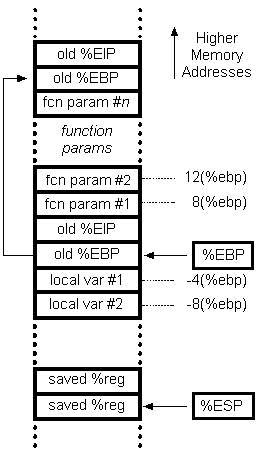
\includegraphics[width=0.4\textwidth]{imgs/stackframe.png}
        \label{fig:stackframe}
        \caption{Stack frame (ia32 - AT\&T notation)}
    \end{figure}	

\end{frame}
